% !TeX root = ../Notizen.tex

\section*{Aufgabe 2: Monte-Carlo-Integration}
In dieser Aufgabe soll eine Monte-Carlo-Integration implementiert werden, dabei ist die Integration wie folgt definiert:
\begin{align}
	\left< f \right> = \int f(x) p(x)dx = \frac{1}{N}\sum\limits_{i} f(x_i)\label{eq:MC-Int}
\end{align}
\subsection*{a)}
Unterverwendung einer Gleichverteilung kann der Flächeninhalt eines Kreises $A_\circ$ bestimmt werden und daraus ein Wert für $\pi$.
Man erzeugt 2 Zufallszahlen aus $x,y\in[0,1]^2$.
Dann wird Bestimmt ob das Paar im Kreis liegt mithilfe von
\begin{align}
	1>x^2+y^2.
\end{align}
Wird dies Häufig genug getan, so wird
\begin{align}
	\frac{A_\circ}{A_\Box}=\frac{{}^\pi\!/\!_4}{1}\approx\frac{N_\circ}{N_\Box}\\
	\Rightarrow \pi \approx 4\frac{N\circ}{N_\Box}
\end{align}
Für $n=10^6$ kommt $\pi\approx 3,14121$ raus.
Diese Methode kann aus \cref{eq:MC-Int} hergeleitet werden.
Dazu wird das Integral
\begin{align}
	\int\limits_{x^2+y^2<1} dx = \frac{1}{N}\sum\limits_{i}f(x_i,y_i)
\end{align}
unter der Wahl von
\begin{align}
f(x_i,y_i)=\begin{cases}
	1\text{ wenn } x_i^2+y_i^2<1\\
	0 \text{ sonst}
\end{cases}
\end{align} \newpage
\subsection*{b)}
Als Relativ Wert wird der vor definiert Wert von C++ verwendet.
Daraus lässt sich ein Fehler in der in Abhängigkeit von der Anzahl an Datenpaaren.
\begin{figure}[h!]
	\centering
	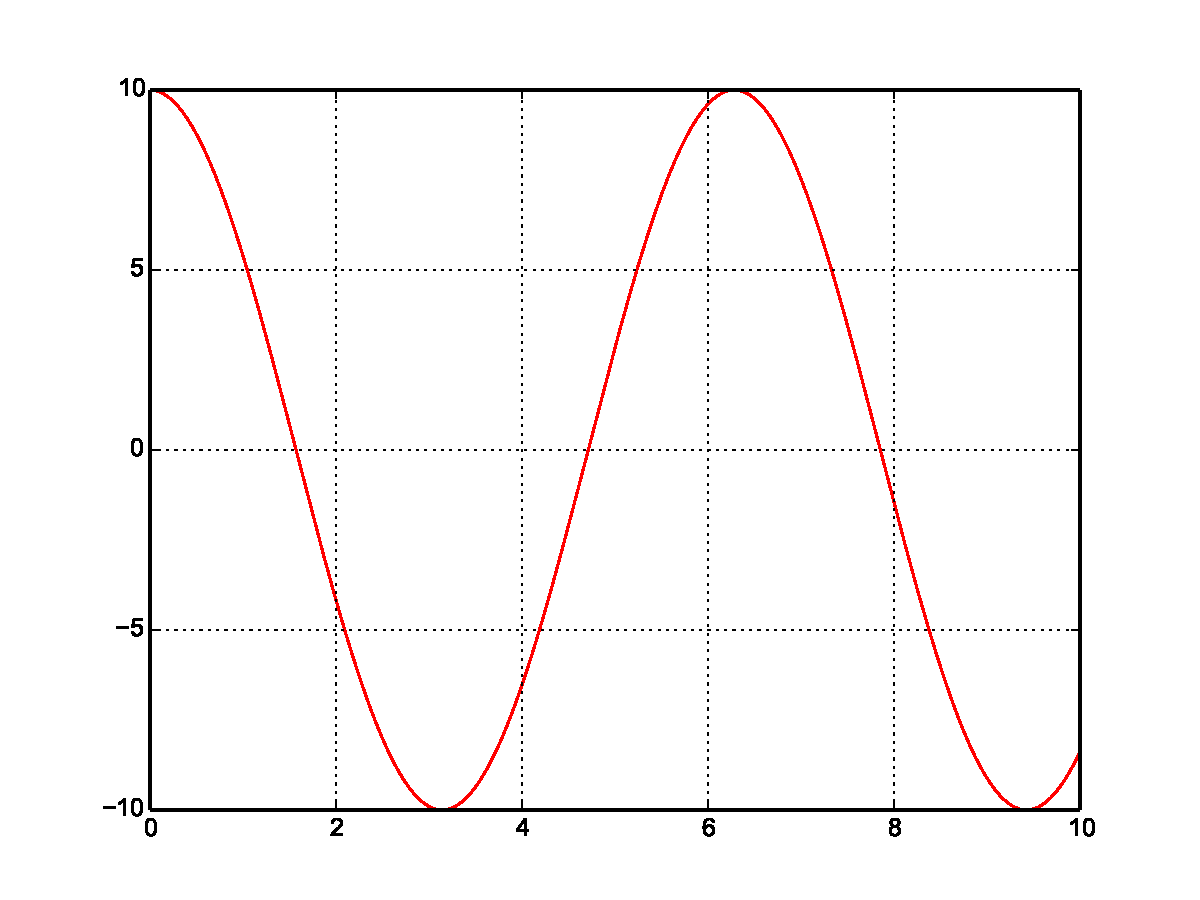
\includegraphics[width = 0.6 \textwidth]{../Plots/Plot_2_A.pdf}
	\caption{Hier ist die relative Abweichung vom Vergleichswert von $\pi$ dargestellt.}
\end{figure} \\
Um eine bessere Schätzung für $\pi$ zu erhalten, wird für 1000 Datenpaare 1000 mal wiederholt. Daraus lässt sich eine Gauß-Verteilung um den Wert $\pi$ erzeugen.
\begin{figure}[h!]
	\centering
	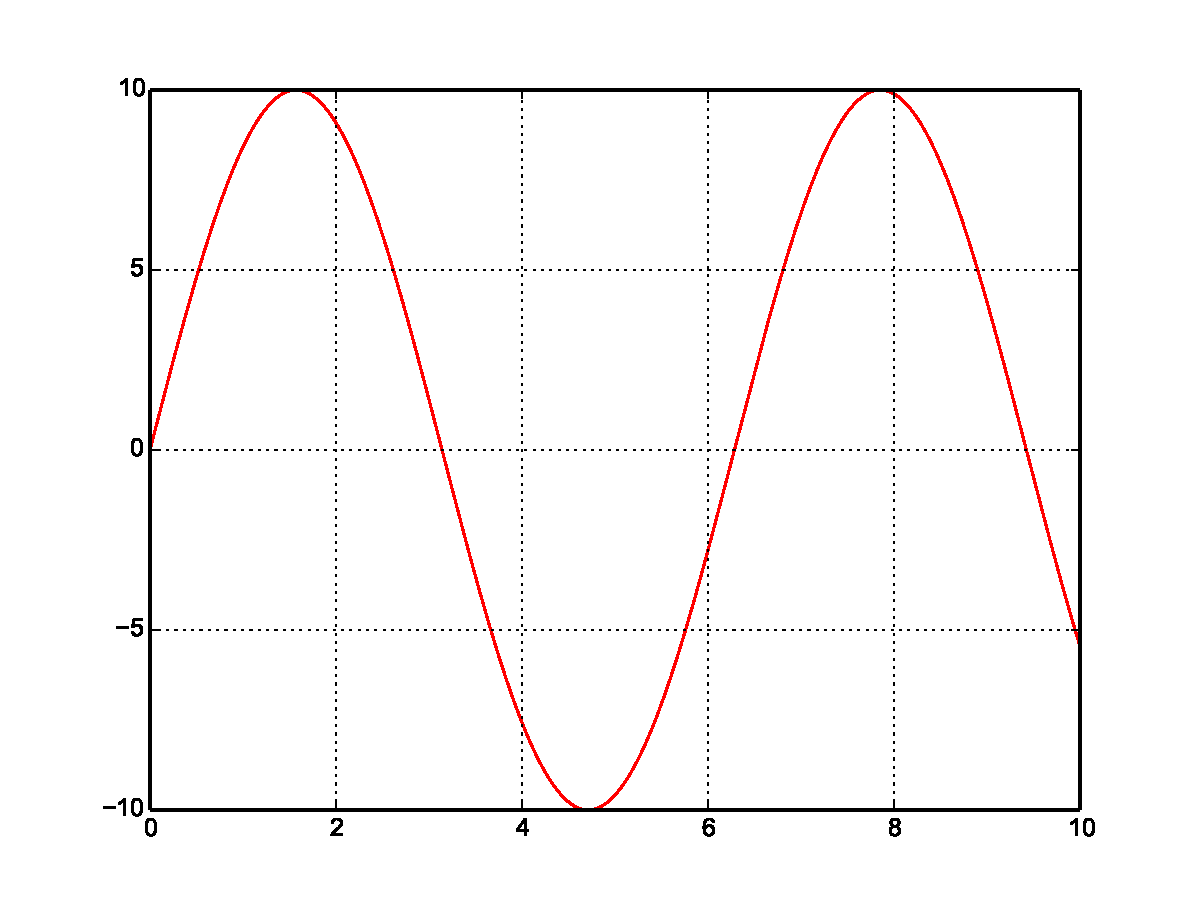
\includegraphics[width = 0.6\textwidth]{../Plots/Plot_2_B.pdf}
	\caption{Hier ist ein Histogramm für 1000 mal Generierung des Wertes für $\pi$ dargestellt.}
\end{figure}\newpage
\subsection*{c)}
Als nächstes wird die Methode benutzt um den Flächeninhalt einer Ellipse zu berechnen.
Dazu wird das Integral
\begin{align}
\int\limits_{(^x\!/\!_a)^2+(^y\!/\!_b)^2<1}dxdy
\end{align}
bestimmt.
Die Bereiche wird, dann zu $x\in[0,a]$ und der $y$-Bereich wird zu $y\in[0,b]$.
Dazu wird $b=1$ gesetzt und für $a\in[0,20]$ der Flächeninhalt berechnet.
Der Flächeninhalt ist 
\begin{align}
	A_\text{Ellpise}=ab\pi
\end{align}
\begin{figure}[h!]
	\centering
	\includegraphics[width = 0.6\textwidth]{../Plots/Plot_2_C.pdf}
	\caption{Hier ist der Flächeninhalt in Abhängigkeit von $a$ dargestellt.}
\end{figure}
\subsection*{d)}
Zum Schluss wird die Monte-Carlo-Integration verwendet um das Integral
\begin{align}
	\int\limits_{(^x^{{}^2}\!/\!_2)+(y)^2<1} e^{-x^2}dxdy
\end{align}
zu berechnen.
Dazu wird die Implementation aus c) verwendet.
Anstelle wird die Funktion
\begin{align}
	f(x_j,y_j)=
	\begin{cases}
		e^{-x^2},\text{ wenn }\frac{x^2}{2}+y^2<1\\
		0\text{ sonst}
	\end{cases}
\end{align}
verwendet.
Der wird dazu 100 mal mit $10^6$ Datenpaaren berechnet um Genauigkeit zu erhöhen und einen Fehler bestimmen zu können.
Die Numerische Lösung ist
\begin{align}
	\int\limits_{(^x^{{}^2}\!/\!_2)+(y)^2<1} e^{-x^2}dxdy=2,99316\pm0,00211
\end{align}